\documentclass[a4paper]{report}

\usepackage[utf8]{inputenc} %Accent
%\usepackage{libertine} %Font
\usepackage[english]{babel} %langue

\usepackage{graphicx} %Include fig
\usepackage{caption} %center the caption
\usepackage{subfig} %Include subfig
\usepackage{lastpage} %ref LastPage 
\usepackage{fancyhdr} % headers,footers
\usepackage{multicol} % minipages
\usepackage{textcomp} 
\usepackage{lscape}   %Format paysage
\usepackage{fancybox} %Image arrière plan
\usepackage{amsmath} %\mathbb, \mathit...
\usepackage{amssymb} 
\usepackage{color} %couleurs
\usepackage{float}
\usepackage[hidelinks]{hyperref} %Liens intradoc et url
\usepackage{titlepic}
\usepackage{tikz} 
%\usepackage{algorithm}
%\usepackage{algorithmic} %Algo en pseudo code
%\usepackage{algorithm2e} %for psuedo code

%\usepackage{boxedminipage} %Surligner

%\newcounter{apppage} % Annexes


%Dossier contenant les figures
\graphicspath{{figures/}}

%Mise en page
\voffset -1.5 cm
\textheight 24.3 cm
\topmargin 0 cm
\headheight 0 cm
%\headsep 0.6 cm
\textwidth 16.5 cm
\evensidemargin 0 cm
\marginparsep 0 cm
\marginparwidth 0 cm
\oddsidemargin -.5 cm


%Type de numérotation des sections & sous-sections
\renewcommand{\thesection}{\Roman{section}}
\renewcommand{\thesubsection}{\thesection.\arabic{subsection}}

%\renewcommand\thesubfigure{(\alph{subfigure})}
\setlength{\parindent}{0cm}
\setlength{\parskip}{1ex plus 0.5ex minus 0.2ex}
\newcommand{\hsp}{\hspace{20pt}}
\newcommand{\HRule}{\rule{\linewidth}{0.5mm}}

%email
\newcommand{\email}[1]{\href{mailto:#1}{\color{blue} \textsf{#1}}}

%Bibliography
\bibliographystyle{apalike}

%Environnement insersion image
\newcommand{\img}[3]{\begin{figure}[!h] \centering \includegraphics[scale=#2]{#1}\captionsetup{justification=centering} \caption{#3} \label{#1} \end{figure}}
  % commande \img{nom image}{scale}{legende}

%TODO
\newcommand{\todo}[1]{{ \Large \textbf{ \colorbox{yellow}{\color{blue} TODO:}}~#1}}

%pushright
\newenvironment{pushright}[1]{\textbf{#1}
\begin{itemize}\item[\hspace{12pt}]}{\end{itemize}
}

\pagestyle{fancy}  % Activation en-tête et pied de page

%En-tête
\fancyhead[L]{}
%\fancyhead[C]{}
%\fancyhead[R]{}
% Pied de page
\newcommand{\width}{3cm}
%\fancyfoot[L]{ \includegraphics[width=\width]{logo-gipsa} }
\fancyfoot[C]{ \thepage~/~\pageref{LastPage} }
%\fancyfoot[R]{ \includegraphics[width=\width]{logo-phelma} }

%\titlepic{\includegraphics[scale=0.6]{kth-logo}}


%LOCAL SHORTCUTS
\newcommand{\ehat}{\hat{\textbf{e}}}
\newcommand{\ey}{\textbf{e}_y}
\newcommand{\ex}{\textbf{e}_x}
\newcommand{\en}{\textbf{e}_n}
\newcommand{\exhat}{ \hat{\textbf{e}}_x }
\newcommand{\zhat}{ \hat{\textbf{z}} }
\newcommand{\scale}{0.4}

%Titre
%\title{Speech Signal Processing\\Report\\Project n°2}
\newcommand{\horrule}[1]{\rule{\linewidth}{#1}} % Create horizontal rule command with 1 argument of height 
%\title{Final Report}

\title{	 
\textsc{EQ2442\\Project Course on Multimedia Signal Processing}\\[25pt] 
\horrule{1pt} \\[0.4cm] % Thin top horizontal rule
\huge {Denoising of MFCCs for better ASR performances} \\[0.4 cm] % The assignment title
\Large{Supervisor: Saikat Chatterjee}\\[0.4 cm]
\horrule{2pt} \\[0.2cm] % Thick bottom horizontal rule
}

\author{ Antoine Honoré\\ \email{honore@kth.se} \and Félix Côte\\\email{fcote@kth.se} }

\begin{document}
%%%%%%%%%%%%%%%% TITLE %%%%%%%%%%%%%%%%
\maketitle
\tableofcontents
%%%%%%%%%%%%%%%%%%%%%%%%%%%%%%%%%%%%%%
\section*{Introduction}
The following document is the final report of a two months project, carried by two master student in signal processing. The goal of this project was to improve the performance of an Automatic Speech Recognition (ASR) by performing a low level denoising on the features extracted from  a speech signal. These features are known as the Mel-Frequency Cepstral Coefficients (MFCCs) and are computed for every frame of a speech signal. These MFCCs are then used as input to train, and to test a SR system. The kick off idea was that, the MFCCs of a frame can be expressed as a linear combination of MFCCs from some other frames. In this report, we will discuss this assumption and try to build a denoising scheme to improve the performance of the SR system.
\section{Background}
\subsection{Feature extraction}
In the case of speech processing, the feature extraction process is not very complicated and is as follow:
\begin{figure}[!ht]
\centering
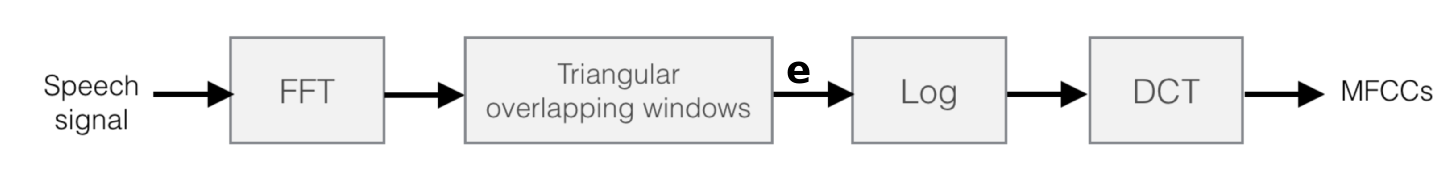
\includegraphics[scale= .3]{feature_extraction}
\caption{MFCCs extraction block diagram}
\label{feature_extraction}
\end{figure}\\
The scheme introduces non-linearity by taking the log of the triangular overlapping windows output. Hence, we are going to work on the output of these overlapping windows. In the rest of the report, we will denote as $\textbf{e} \in \mathbb{R}^M$ this vector. Here M = 26.

\subsection{Pattern recognition with kaldi}
To test our denoising scheme, we used kaldi, a free and open-source sofware. Kaldi is an implementation of all the tools that we need to compute MFCCs, train and test a pattern recognition model. Here we chose to drop the MFCCs computation implemented in Kaldi and created our own implemented with Matlab. The pattern recognition system that we used is based on Hidden Markov Model and the probability distribution of the states are modeled with GMM.

\subsection{Database}
We used the TIMIT database to train and test our system. The kaldi implementation provides testing examples on different databases and TIMIT is one of them. We therefore had access to the implementation of the scoring process using the TIMIT database and that saved us a lot of time.

\section{Denoising algorithm}
The idea is to reduce the dimension of \textbf{e} and find a vector $\ehat = \sum_{i=1}^N\textbf{d}_iz_i$ . Here, $\textbf{d}_i$ is the ith column of a fat matrix D and is used as a codebook. To reduce the dimension, \textbf{z} has have strictly less than M non-zero coefficients.
We denote by x the clean speech signal, n the additive noise and y = x + n, the noisy signal. 
First we assume that the additivity holds up to the mel coefficients, $\ey= \ex + \en$.\\
The problem is the following:\\
we want to find a sparsed vector \textbf{z} such that $||\ey-D\textbf{z}||_2 \leq \epsilon$ and $D\mathbf{z} > 0$. If $\epsilon$ is well chosen, we will have $||\ex - \exhat||_2 \leq ||\ex - \ey||_2$

\subsection{Computation of a codebook D}

\subsection{Sparse vector}
The sparsity of a vector can be measured with the $\ell^0$-norm. We could hence formulate the following problem:

\begin{equation}
  \begin{aligned}
    & \underset{\mathbf{z}}{\text{minimize}}
    & & ||\mathbf{z}||_0 \\
    & \text{subject to}
    & & ||\ey -D\mathbf{z}||_2 \leq \epsilon\\
    &&& -D\mathbf{z} \leq \eta
  \end{aligned}
\label{l0}
\end{equation}

%minimize $||\mathbf{z}||_0$\\subject to $||\ey -D\mathbf{z}||_2 \leq \epsilon$\\

However, $\ell^0-norm$ is a pseudo-norm, hence the problem is consider not tractable. \cite{equivalencel1l0} shows that the solution of the problem:
\begin{equation}
  \begin{aligned}
    & \underset{\mathbf{z}}{\text{minimize}}
    & & ||\mathbf{z}||_1 \\
    & \text{subject to}
    & & ||\ey -D\mathbf{z}||_2 \leq \epsilon\\
    &&& -D\mathbf{z} \leq \eta
  \end{aligned}
\label{l1}
\end{equation}
 is often a good approximation of the solution of problem \ref{l0}. Problem \ref{l1} is convex and is therefore easier and faster to solve.\\
Ideally $\eta = 0$. However, for (\ref{l1}) to remain a convex optimization problem, the inequality constraint must not be strict. In our case, we want the approximated mel coefficients to be strictly positive, therefore we chose $\eta = 10^{-4}$. This value represents the lower value that the mel coefficients can now take.
%Let define $\zhat$ as the solution of problem \ref{l1}.
The solver we used is CVX\footnote{CVX documentation: http://web.cvxr.com/cvx/doc/}.\\

With the CVX syntax, the problem looks like this:
\img{convex_problem}{.7}{Convex problem with CVX syntax}


\subsection{Silence frames}
We need to separate two types of frames:\begin{enumerate}
\item the speech frames (high energy) containing the information;
\item the silence frames (low energy) containing  noise. \end{enumerate}

There is a big difference of structure between these frames and hence it is not possible to process them the same way.
On figure \ref{speechMC} and \ref{silMC} we see the difference  between two speech and two silence frames.

\begin{figure}[!ht]
\subfloat[Mel coefficients of a speech frame]{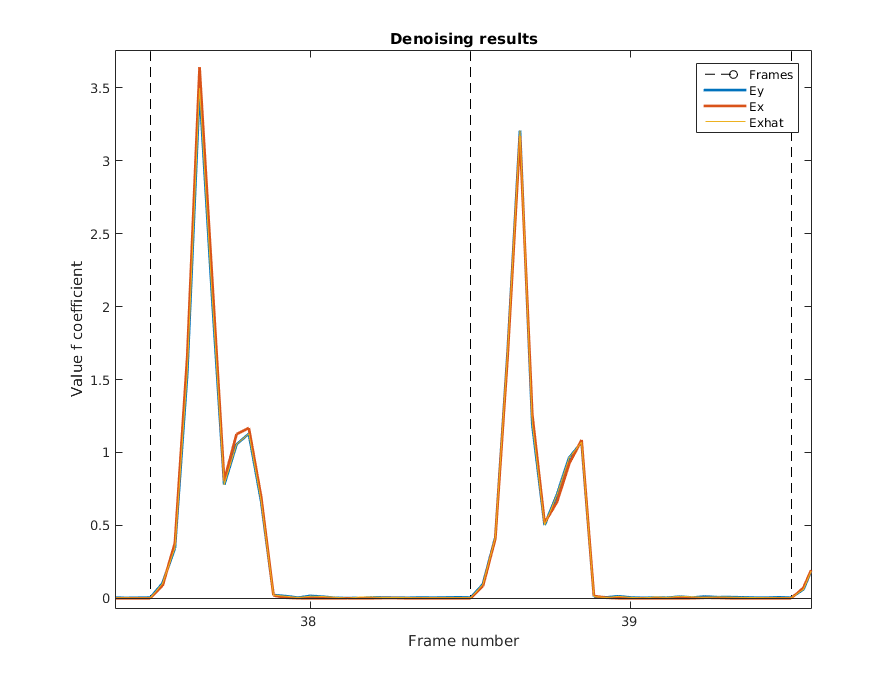
\includegraphics[scale=.38]{speechframeMC}\label{speechMC}}
\subfloat[Mel coefficients of a silence frame. Here we did not process the silence so $\exhat=\ey$]{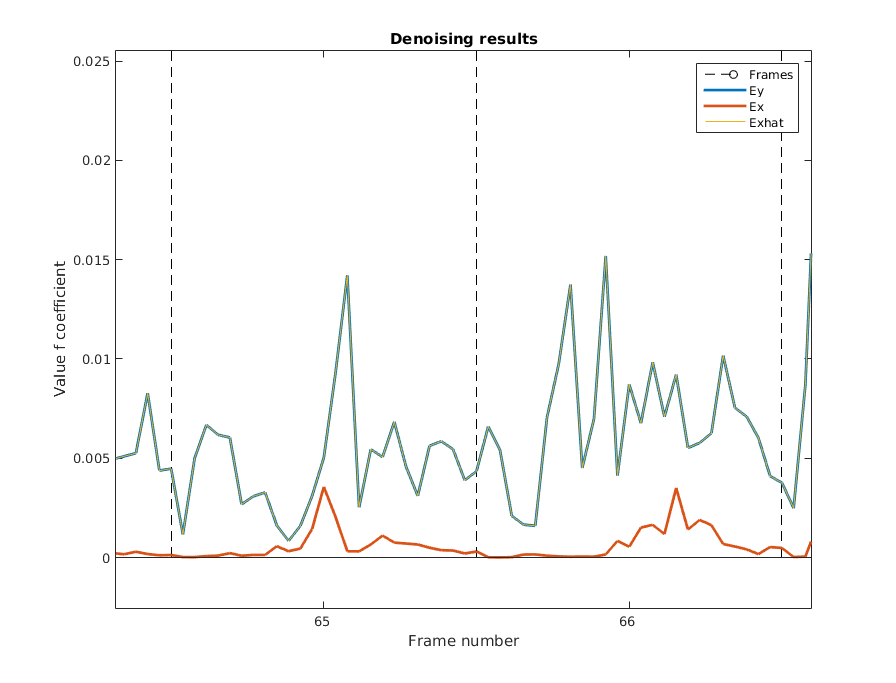
\includegraphics[scale=.38]{silenceframeMC}\label{silMC}}\\
\caption{Difference between speech \& silence frames.}
\end{figure}

An  easy, cheap and efficient solution that we found to process the silence frame is to use a simple spectral substraction.
Since this part of the denoising algorithm was not really a part of the project I won't say more but the result can be seen on figure \ref{kaldiperformances}.



\pagebreak
\section{Results}
\subsection{Additivity hypothesis}

\subsection{Reducing the dimension}

\begin{figure}[!ht]
\centering
     \subfloat[$\epsilon=0.001$]{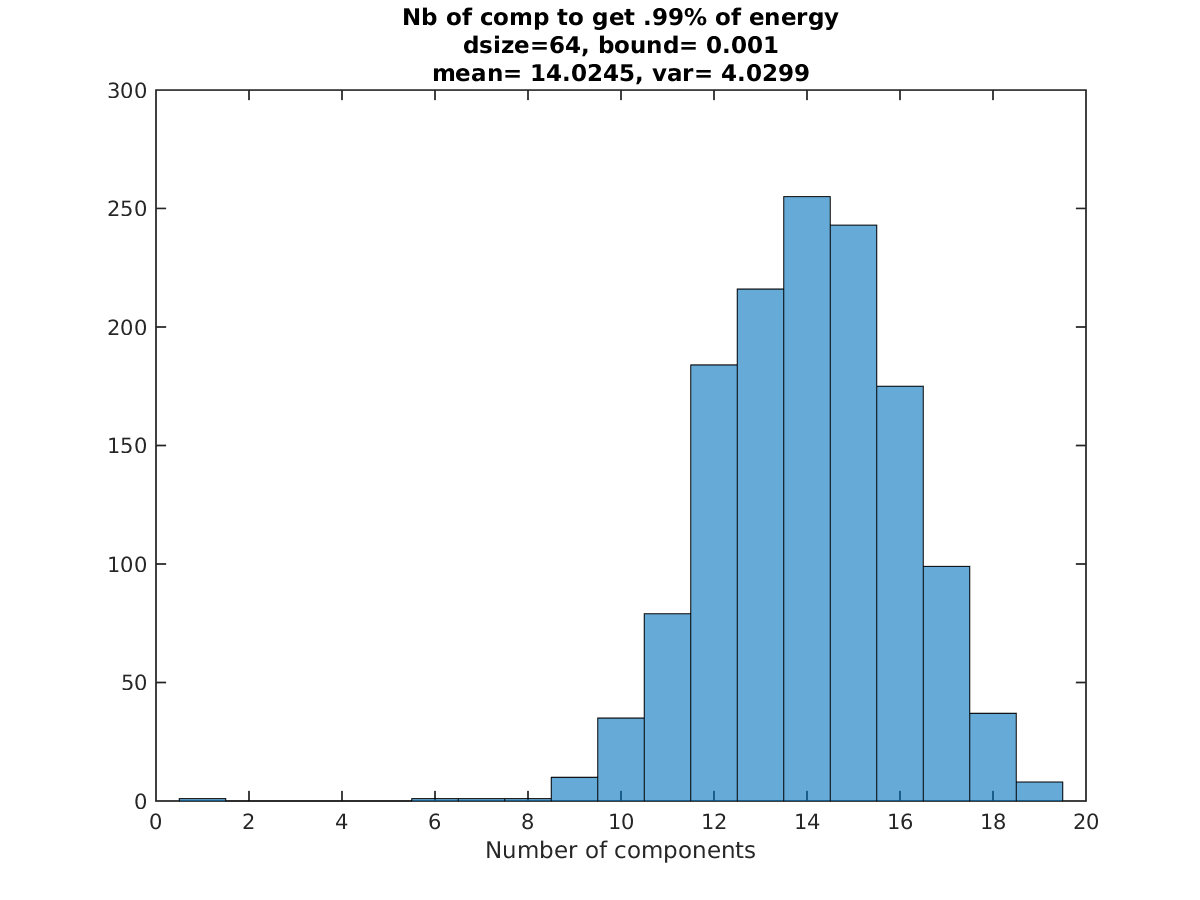
\includegraphics[scale=\scale]{sparsity_dsize64_bound0_001}\label{b0.001}}
     \subfloat[$\epsilon=0.005$]{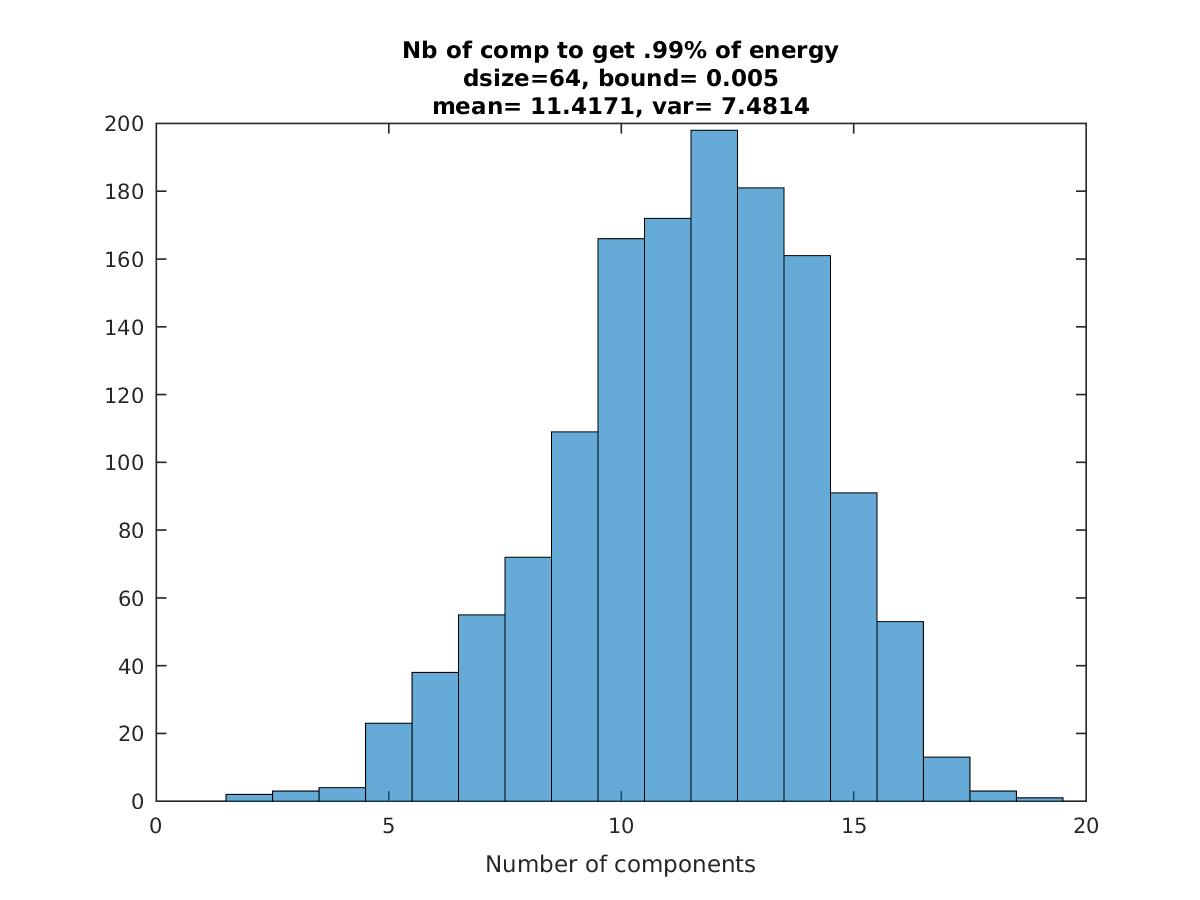
\includegraphics[scale=\scale]{sparsity_dsize64_bound0_005}\label{b0.005}}\\
     \subfloat[$\epsilon=0.01$]{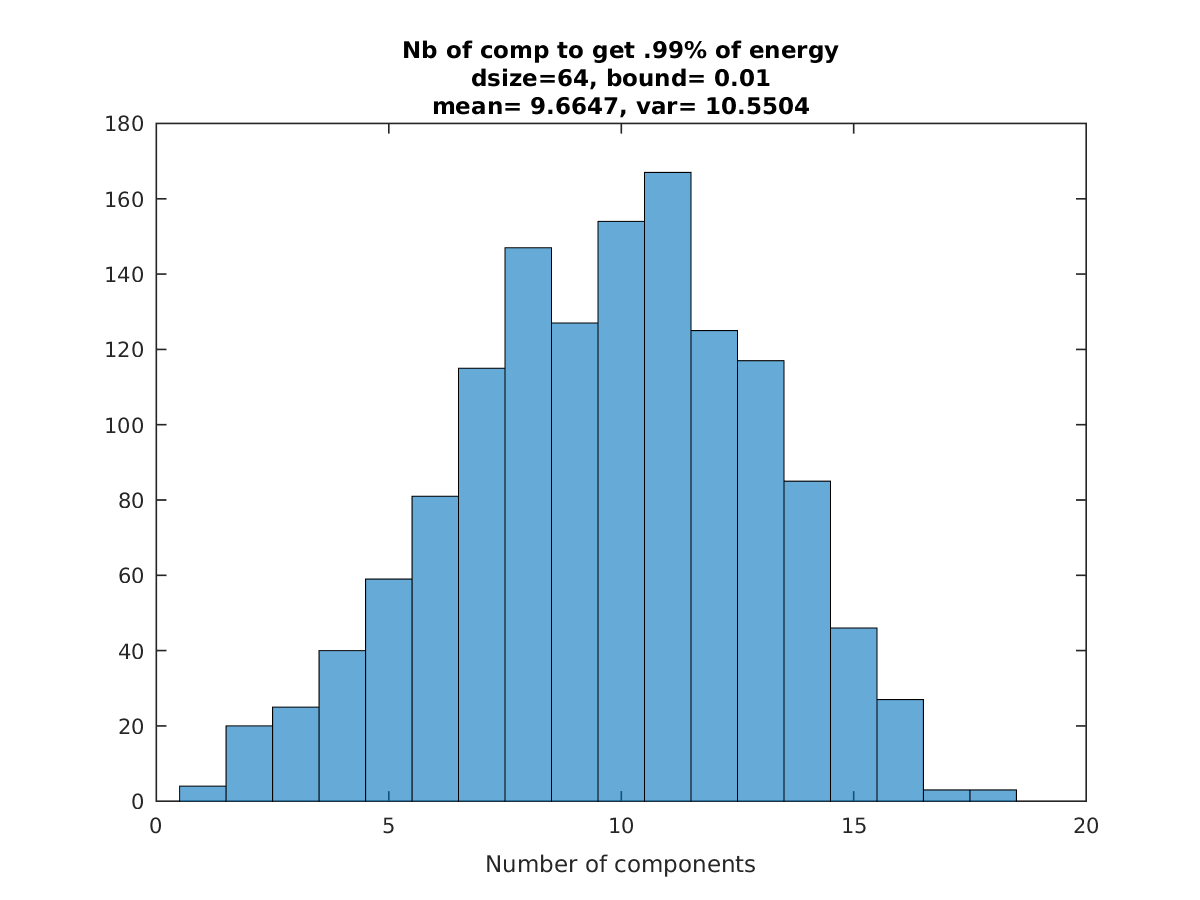
\includegraphics[scale=\scale]{sparsity_dsize64_bound0_01}\label{b0.01}}
     \subfloat[$\epsilon=0.02$]{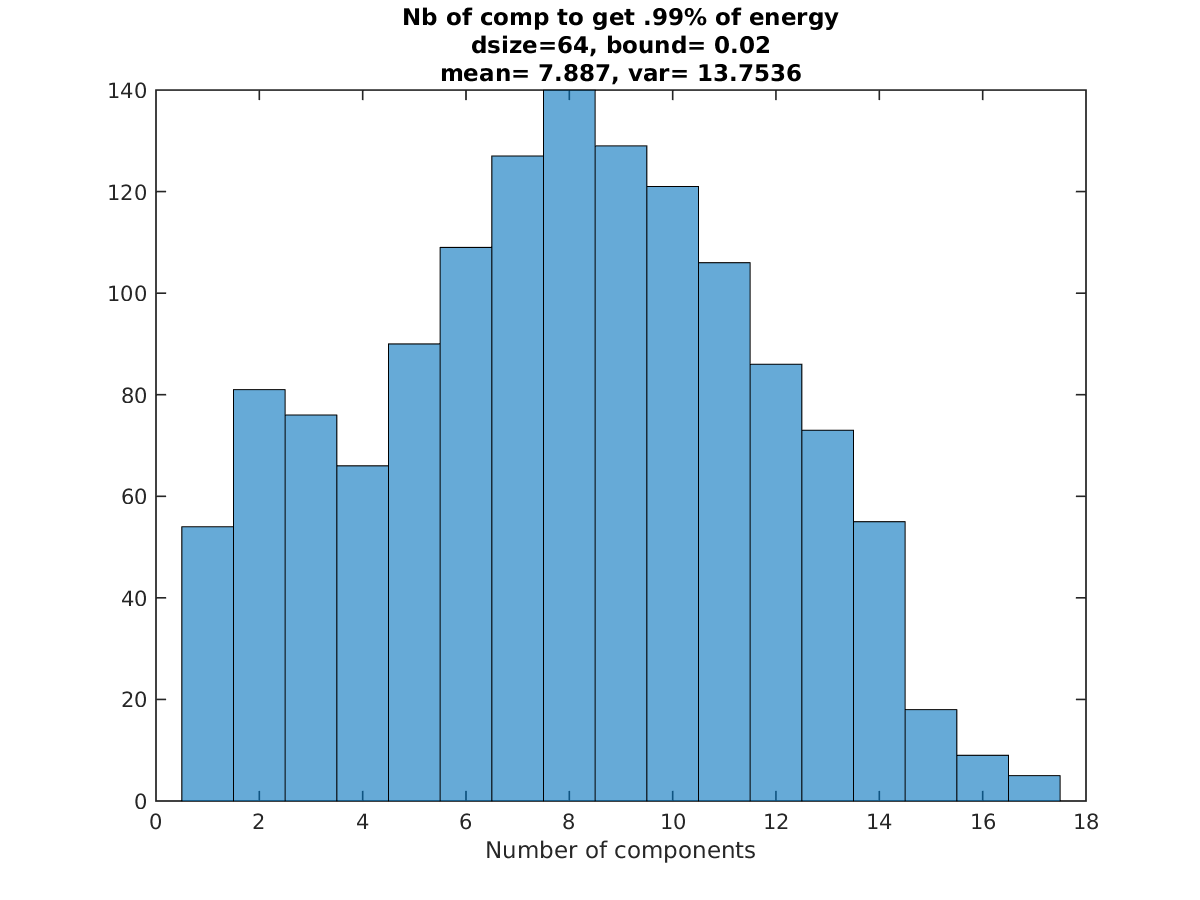
\includegraphics[scale=\scale]{sparsity_dsize64_bound0_02}\label{b0.02}}\\
     \subfloat[$\epsilon=0.05$]{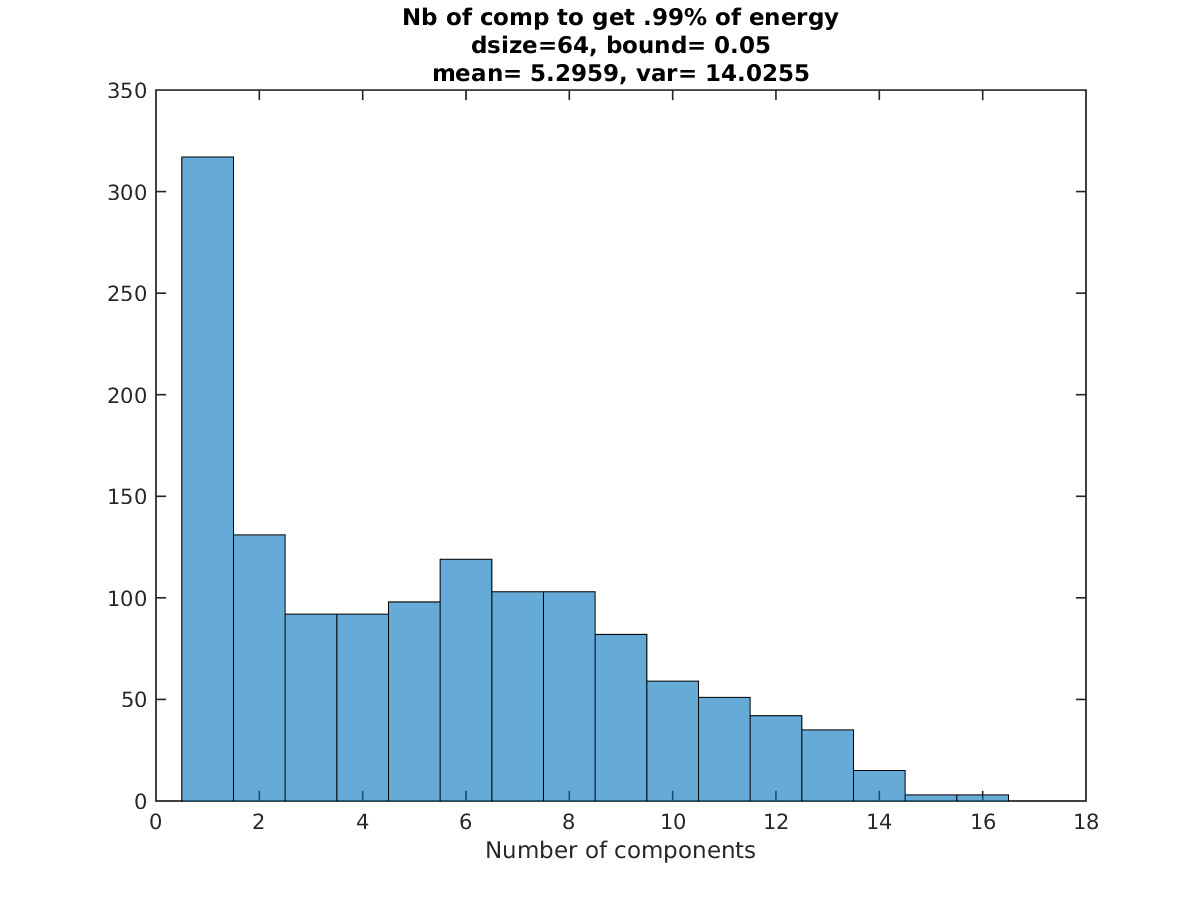
\includegraphics[scale=\scale]{sparsity_dsize64_bound0_05}\label{b0.05}}
     \subfloat[$\epsilon=0.1$]{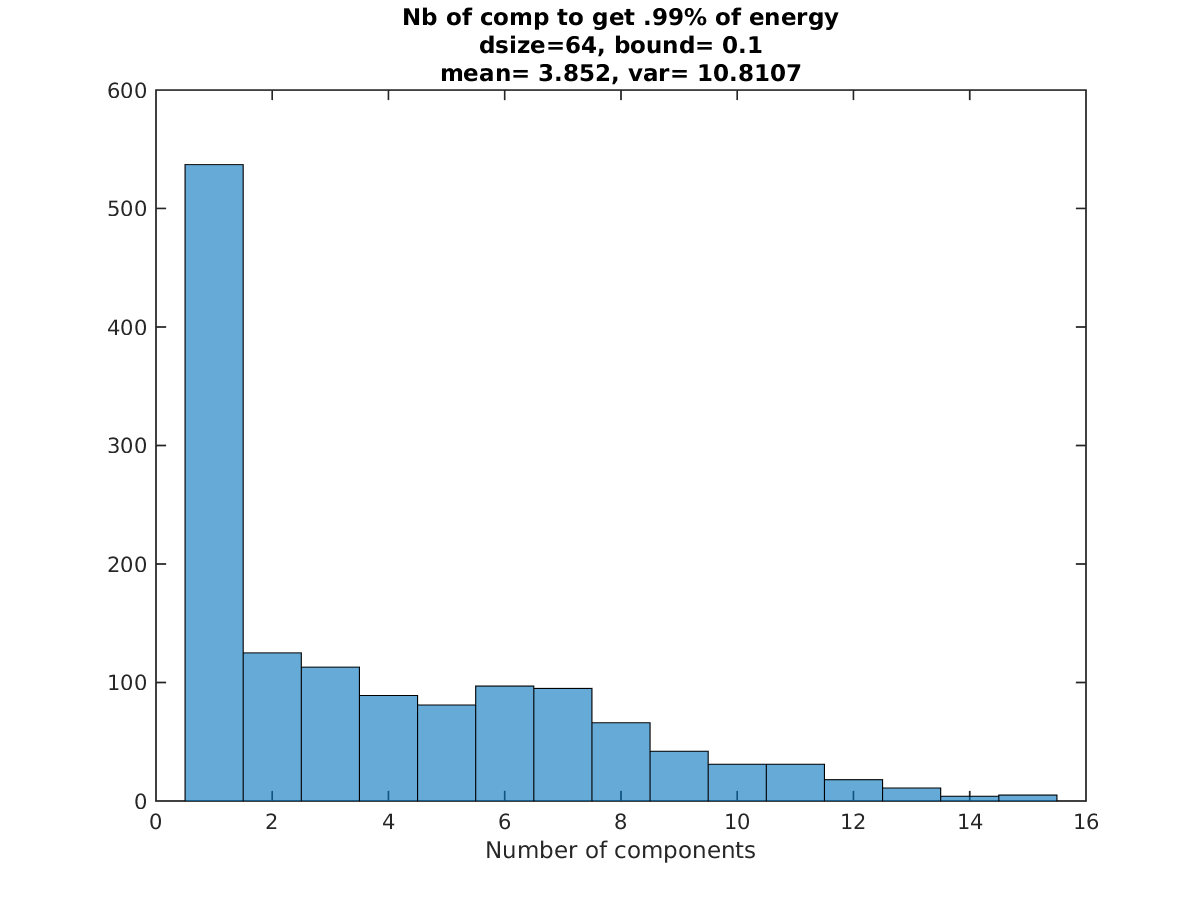
\includegraphics[scale=\scale]{sparsity_dsize64_bound0_1}\label{b0.1}}\\
     \caption{Number of components necessary to represent 99\% of the energy of $\zhat$. There is one $\zhat$ for every frame and we processed $\approx$ 1500 frames. Here $\zhat \in \mathbb{R}^{64}$}
     \label{histogram}
\end{figure}
Figure \ref{sparseparam} shows the evolution of the mean of the variance of the histogram of figure \ref{histogram} when we vary $\epsilon$. We computed these two curves (mean and variance) for different sizes of the dictionnary. 

\begin{figure}[!ht]
\centering
\subfloat[]{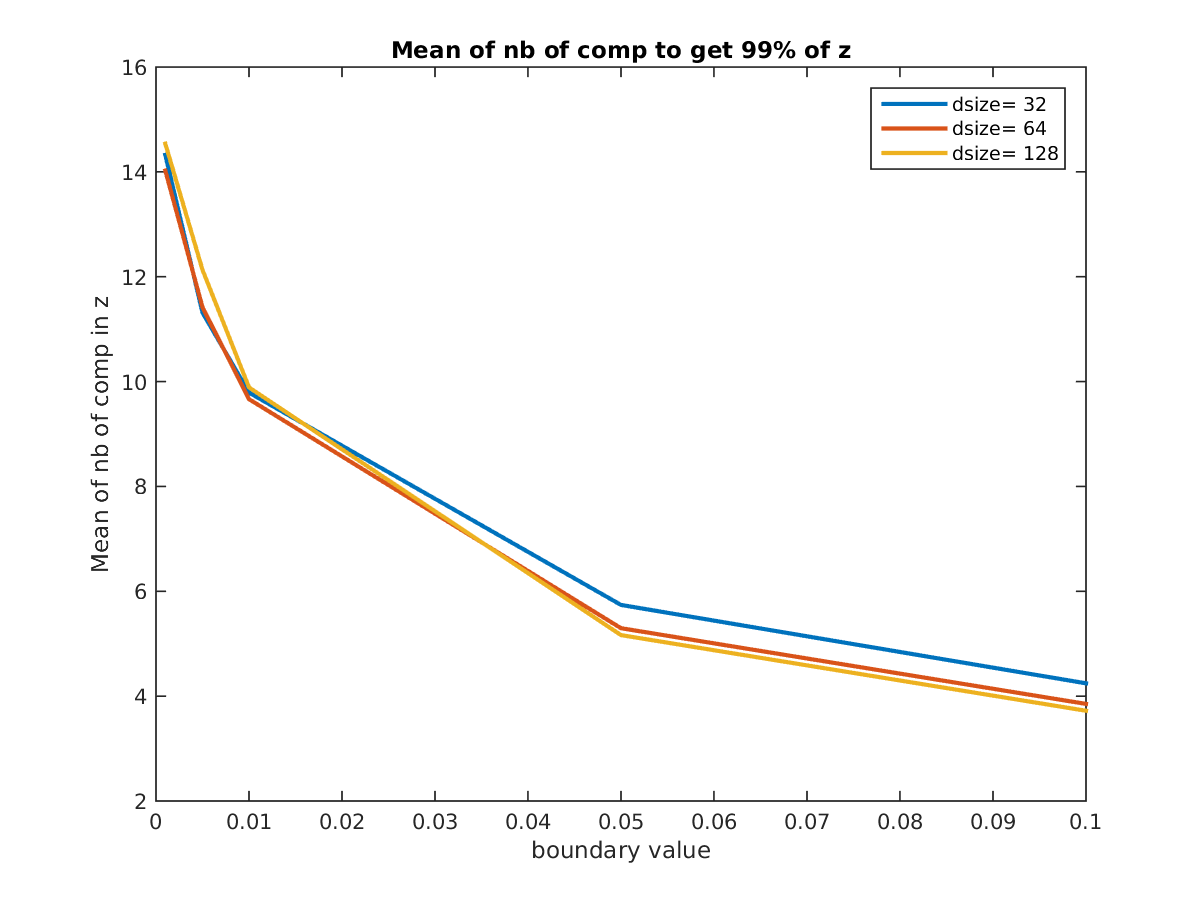
\includegraphics[scale=\scale]{sparsity_mean}\label{sparsemean}}
\subfloat[]{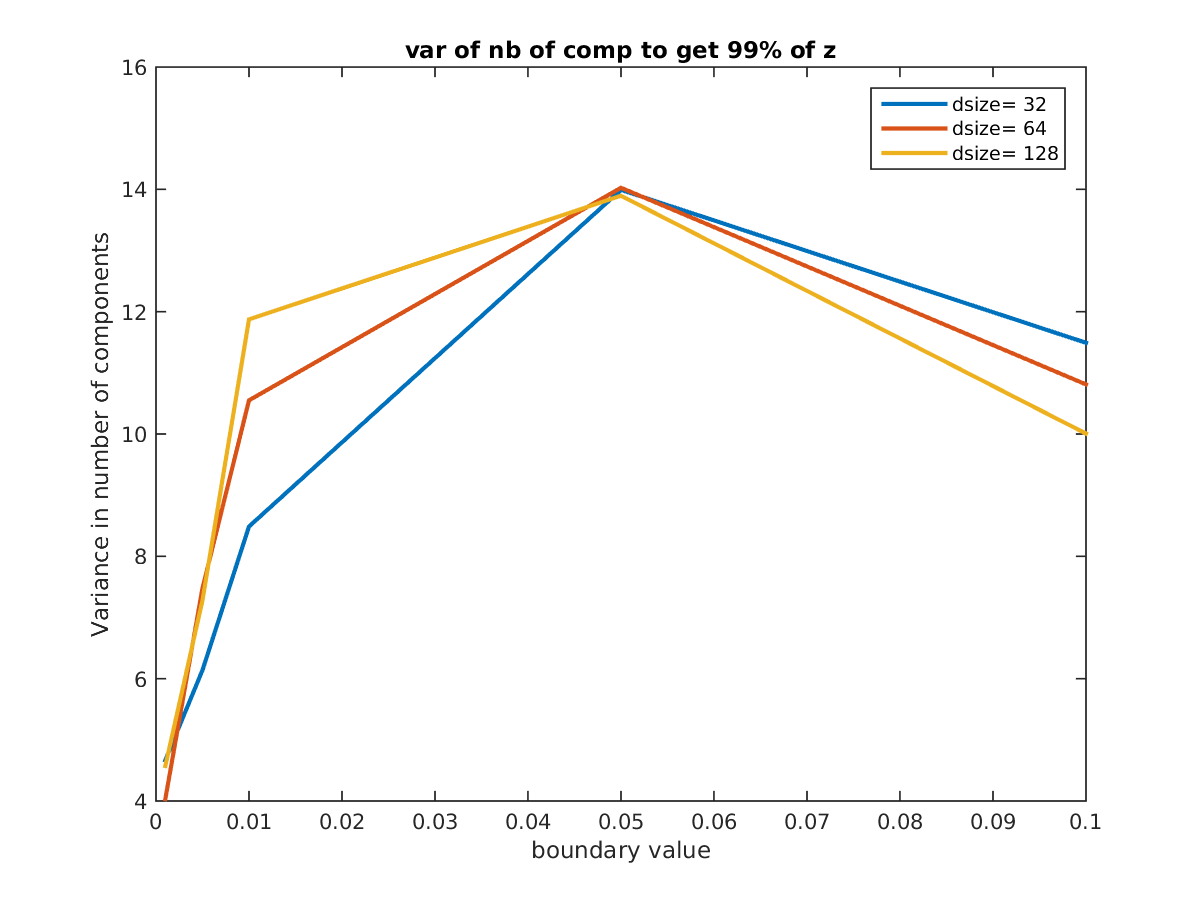
\includegraphics[scale=\scale]{sparsity_variance} \label{sparsevar} }
\caption{}
\label{sparseparam}
\end{figure}

\subsection{Kaldi performances}


As figure \ref{kaldiperformances} shows, the denoising algorithm does not improve kaldi's performances.
\img{kaldiperformances}{.5}{Plot of kaldi performances versus value of $\epsilon$ for different kinds of processing.}

We observe that we do not manage to fit $\ex$ by allowing $||\ey-\exhat||_2$ to become large.


\bibliography{bibtex}
\end{document}
%%% Local Variables:
%%% TeX-master: "master"
%%% End:
